\documentclass[hyperref]{ctexart}
\usepackage[left=2.50cm, right=2.50cm, top=2.50cm, bottom=2.50cm]{geometry} %页边距
\usepackage{helvet}
\usepackage{amsmath, amsfonts, amssymb} % 数学公式、符号
\usepackage[english]{babel}
\usepackage{graphicx}   % 图片
\usepackage{url}        % 超链接
\usepackage{bm} 
\usepackage{graphicx}        % 加粗方程字体
\usepackage{multirow}
\usepackage{booktabs}
\usepackage{algorithm}
\usepackage{algorithmic}
\renewcommand{\algorithmicrequire}{ \textbf{Input:}}       
\renewcommand{\algorithmicensure}{ \textbf{Initialize:}} 
\renewcommand{\algorithmicreturn}{ \textbf{Output:}}     
%算法格式
\usepackage{fancyhdr} %设置页眉、页脚
\pagestyle{fancy}
\lhead{CN}
\chead{{\Large \textbf{说\hspace{1em}明\hspace{1em}书\hspace{1em}附\hspace{1em}图}}}
\rhead{1/2}
\usepackage{hyperref} %bookmarks
\hypersetup{colorlinks, bookmarks, unicode} %unicode
\usepackage{multicol}
\usepackage{indentfirst} %%缩进

\begin{document}
	
	xxx
	\thispagestyle{empty}
	\clearpage
	\setcounter{page}{6}	
	
	\begin{figure}[htbp]
		\qquad		\qquad	\qquad	\qquad	\qquad		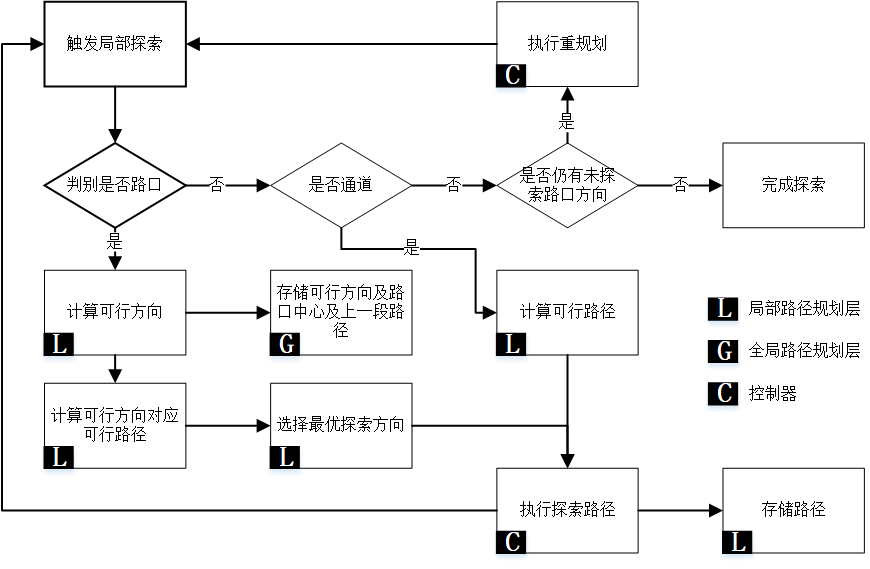
\includegraphics[width=0.6\linewidth]{graph/structure.png}
		\begin{center}
			图4
		\end{center}
		\label{fig:04}
		\begin{center}
			\quad	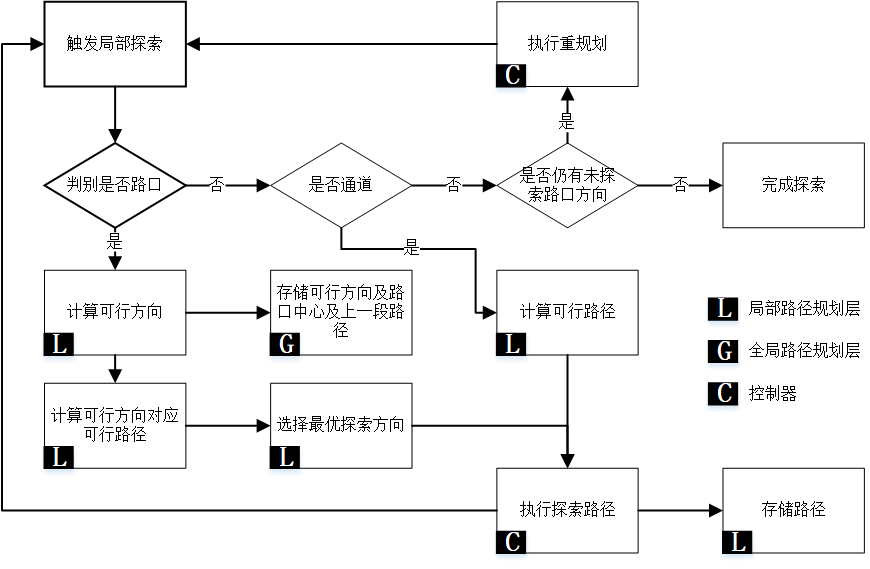
\includegraphics[width=0.6\linewidth]{graph/structure.png}
			\begin{center}图5\end{center}
		\label{fig:05}
		\end{center}
	\end{figure}
	



	
	
	
	
	
	
	
	
	
	
	
	
\end{document}